% Ch4: the four VAE adaptation strategies (Group 1), trainable vs frozen.
% Matches VaeTrainer._load_vae:
%   Color adapter  (mode=adapter): 1x1 in/out adapters (4->3, 3->4) + decoder train; RGB encoder frozen.
%   Decoder-only   (inflate, freeze_conv_in, trunk frozen): conv_in grown to 4 ch (new slot zero-init) but frozen.
%   Input+Decoder  (inflate, conv_in trainable, trunk frozen).
%   Full FT        (inflate, conv_in + whole encoder trunk trainable).
% The decoder (incl. its conv_out) trains in every strategy.
\documentclass[tikz,border=4pt]{standalone}
\usepackage{amsmath,amssymb}
\usetikzlibrary{arrows.meta,positioning,calc}
% Shared colours for the thesis TikZ figures. Same reference palette as
% scripts/thesis_figures.py (dataviz light mode), so diagrams and plots match.
\definecolor{ink}{HTML}{0B0B0B}
\definecolor{ink2}{HTML}{52514E}
\definecolor{muted}{HTML}{898781}
\definecolor{hair}{HTML}{C3C2B7}
\definecolor{neutralfill}{HTML}{F0EFEC}
\definecolor{blue}{HTML}{2A78D6}
\definecolor{bluefill}{HTML}{CDE2FB}
\definecolor{bluedark}{HTML}{184F95}
\definecolor{orange}{HTML}{EB6834}
\definecolor{orangefill}{HTML}{FBE0D3}
\definecolor{aqua}{HTML}{1BAF7A}
\definecolor{aquafill}{HTML}{D2F0E4}
\definecolor{violet}{HTML}{4A3AA7}
\definecolor{violetfill}{HTML}{E3E0F6}

% Trainable modules: orange fill + solid border. Frozen: neutral fill,
% dashed border, and every figure also labels the state in text.
\tikzset{
  every node/.style={font=\small, text=ink},
  box/.style={draw=hair, rounded corners=2pt, align=center, inner sep=4pt, line width=0.6pt},
  trainable/.style={box, fill=orangefill, draw=orange, line width=0.8pt},
  frozen/.style={box, fill=neutralfill, draw=muted, dashed},
  data/.style={box, fill=bluefill, draw=blue},
  latent/.style={box, fill=violetfill, draw=violet},
  cond/.style={box, fill=aquafill, draw=aqua},
  arr/.style={-{Stealth[length=5pt]}, draw=ink2, line width=0.7pt},
  note/.style={font=\footnotesize, text=ink2, align=center},
}


\begin{document}
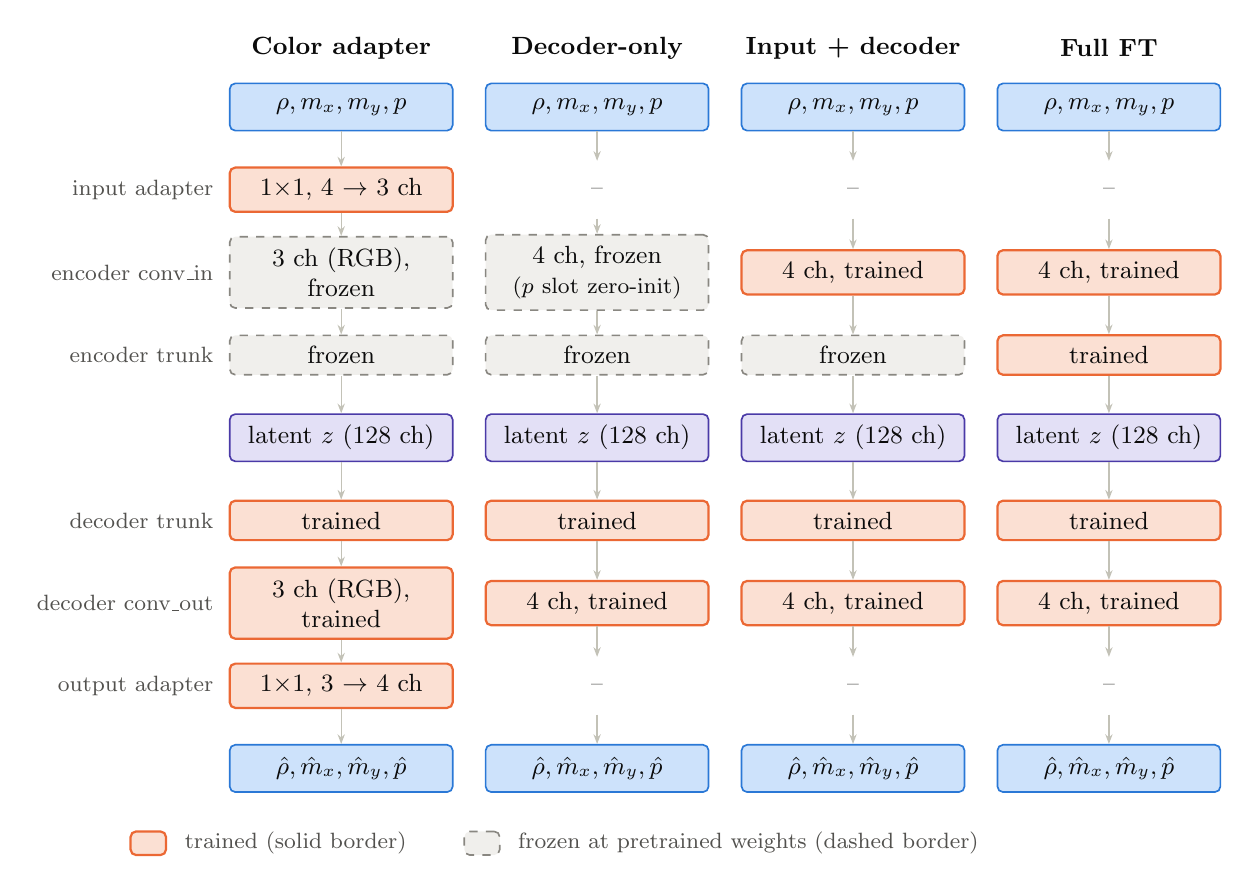
\begin{tikzpicture}
  \def\colw{3.25}
  % rows: y positions
  \def\yin{0}      \def\yad{-1.05}  \def\yci{-2.1}  \def\ytr{-3.15}
  \def\ylat{-4.2}  \def\ydec{-5.25} \def\yco{-6.3}  \def\yoa{-7.35} \def\yout{-8.4}

  % row labels
  \foreach \y/\t in {\yad/input adapter, \yci/encoder conv\_in, \ytr/encoder trunk, \ydec/decoder trunk, \yco/decoder conv\_out, \yoa/output adapter} {
    \node[note, anchor=east] at (1.15,\y) {\t};
  }

  % column titles
  \foreach \i/\t in {1/Color adapter, 2/Decoder-only, 3/Input + decoder, 4/Full FT} {
    \node[font=\small\bfseries] at (\i*\colw-0.6, 0.75) {\t};
  }

  \foreach \i in {1,...,4} {
    \pgfmathsetmacro{\x}{\i*\colw-0.6}
    \node[data, minimum width=2.75cm, text width=2.55cm, minimum height=0.6cm] (in\i) at (\x,\yin) {$\rho, m_x, m_y, p$};
    \node[latent, minimum width=2.75cm, text width=2.55cm, minimum height=0.6cm] (lat\i) at (\x,\ylat) {latent $z$ (128 ch)};
    \node[data, minimum width=2.75cm, text width=2.55cm, minimum height=0.6cm] (out\i) at (\x,\yout) {$\hat\rho, \hat m_x, \hat m_y, \hat p$};
  }

  % --- column 1: color adapter --------------------------------------------
  \pgfmathsetmacro{\x}{1*\colw-0.6}
  \node[trainable, minimum width=2.75cm, text width=2.55cm] (a1) at (\x,\yad) {1$\times$1, 4 $\to$ 3 ch};
  \node[frozen,    minimum width=2.75cm, text width=2.55cm] (b1) at (\x,\yci) {3 ch (RGB), frozen};
  \node[frozen,    minimum width=2.75cm, text width=2.55cm] (c1) at (\x,\ytr) {frozen};
  \node[trainable, minimum width=2.75cm, text width=2.55cm] (d1) at (\x,\ydec) {trained};
  \node[trainable, minimum width=2.75cm, text width=2.55cm] (e1) at (\x,\yco) {3 ch (RGB), trained};
  \node[trainable, minimum width=2.75cm, text width=2.55cm] (f1) at (\x,\yoa) {1$\times$1, 3 $\to$ 4 ch};

  % --- columns 2-4: inflated VAE, no adapters -------------------------------
  \foreach \i/\ci/\cis/\tr/\trs in {
      2/frozen/{4 ch, frozen\\\footnotesize ($p$ slot zero-init)}/frozen/frozen,
      3/trainable/{4 ch, trained}/frozen/frozen,
      4/trainable/{4 ch, trained}/trainable/trained} {
    \pgfmathsetmacro{\x}{\i*\colw-0.6}
    \node[note, minimum width=2.75cm, minimum height=0.72cm] (a\i) at (\x,\yad) {--};
    \node[\ci, minimum width=2.75cm, text width=2.55cm] (b\i) at (\x,\yci) {\cis};
    \node[\tr, minimum width=2.75cm, text width=2.55cm] (c\i) at (\x,\ytr) {\trs};
    \node[trainable, minimum width=2.75cm, text width=2.55cm] (d\i) at (\x,\ydec) {trained};
    \node[trainable, minimum width=2.75cm, text width=2.55cm] (e\i) at (\x,\yco) {4 ch, trained};
    \node[note, minimum width=2.75cm, minimum height=0.72cm] (f\i) at (\x,\yoa) {--};
  }

  % vertical flow arrows
  \foreach \i in {1,...,4} {
    \foreach \u/\v in {in/a, a/b, b/c, c/lat, lat/d, d/e, e/f, f/out} {
      \draw[-{Stealth[length=3.5pt]}, draw=hair, line width=0.5pt] (\u\i.south) -- (\v\i.north);
    }
  }

  % legend
  \node[trainable, minimum width=0.45cm, minimum height=0.3cm, inner sep=0pt] (l1) at (0.2,-9.35) {};
  \node[note, right=0.1cm of l1, anchor=west] (l1t) {trained (solid border)};
  \node[frozen, minimum width=0.45cm, minimum height=0.3cm, inner sep=0pt, right=0.6cm of l1t] (l2) {};
  \node[note, right=0.1cm of l2, anchor=west] {frozen at pretrained weights (dashed border)};
\end{tikzpicture}
\end{document}
